\section{Fast re-planning for moving obstacle avoidance}

\begin{figure}[ht]
  \begin{center}
  \begin{tikzpicture}
    \node[anchor=south west,inner sep=0] (image) at (0,0){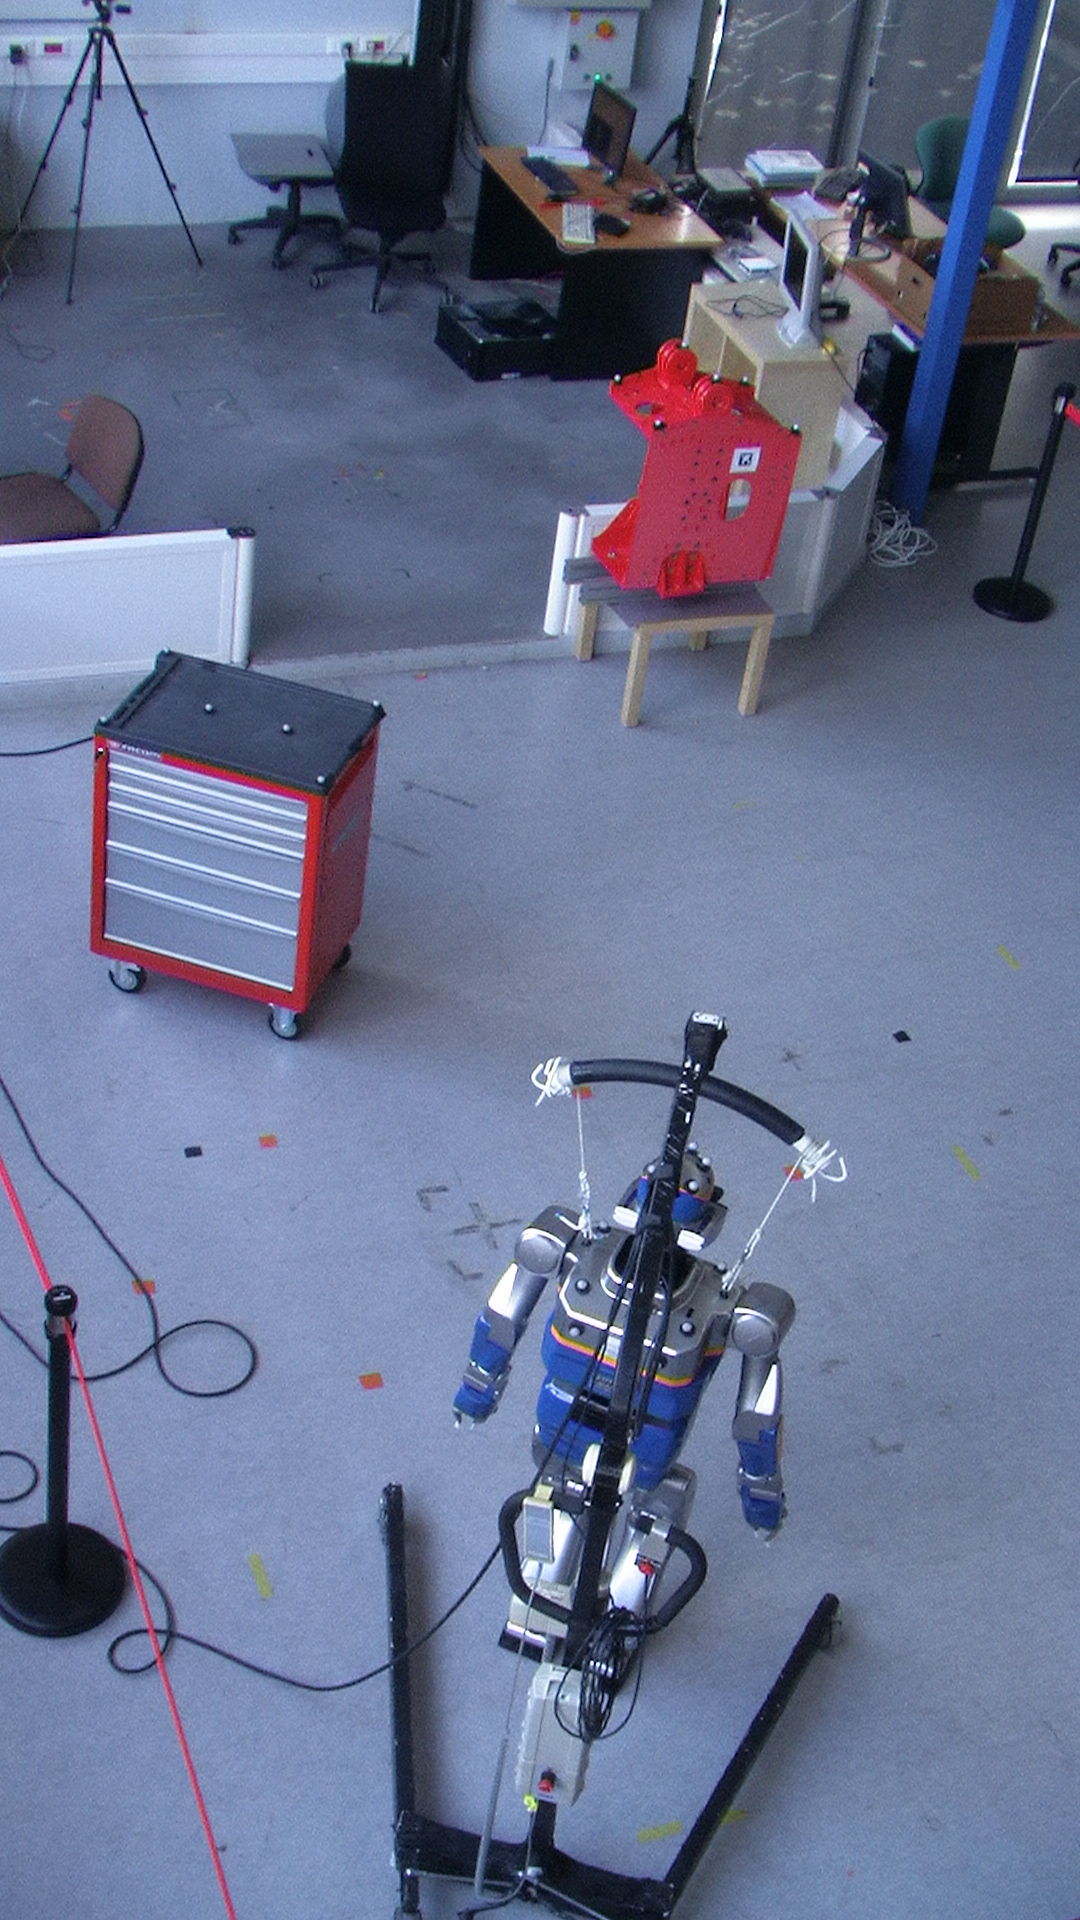
\includegraphics[height=0.5\linewidth]{./figures/SituationFastPlanning_2.jpg}};
    \begin{scope}[x={(image.south east)},y={(image.north west)}]
        \draw[blue,ultra thick,rounded corners] (0.53,0.68) rectangle (0.75,0.83);
        \draw[red,ultra thick,rounded corners] (0.06,0.45) rectangle (0.37,0.67);
        %\draw[help lines,xstep=.1,ystep=.1] (0,0) grid (1,1);
    \end{scope}
  \end{tikzpicture} \hspace*{2cm}
  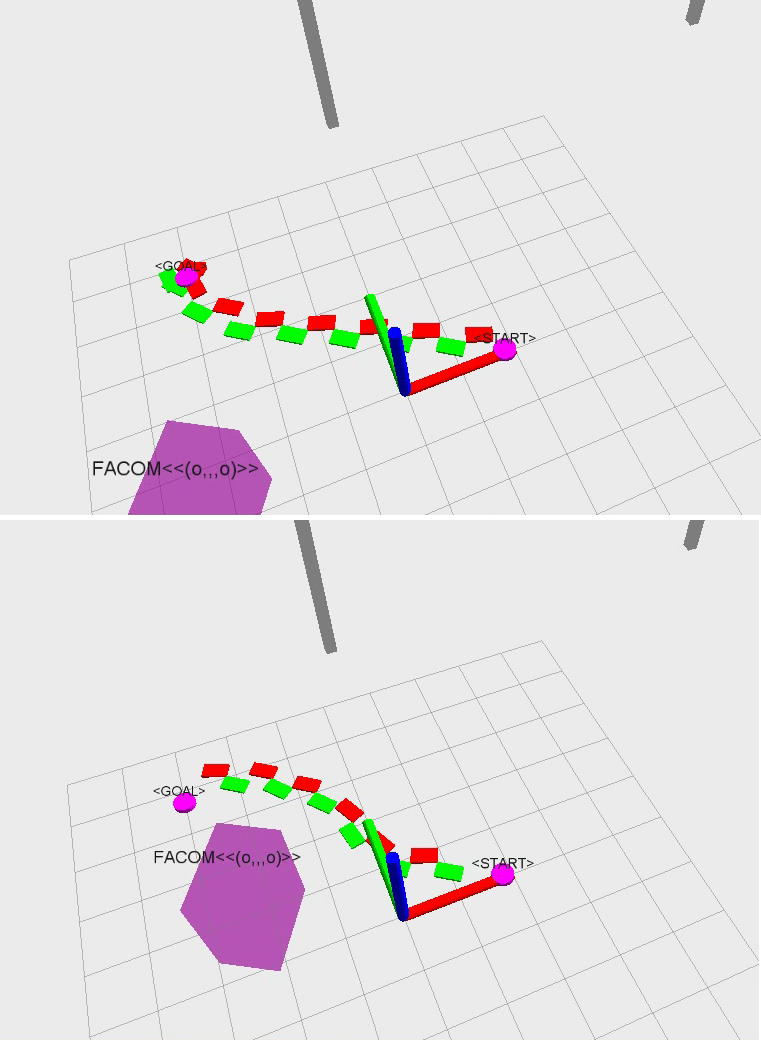
\includegraphics[height=0.5\linewidth]{./figures/Replanning-Start-End.png}
  \caption{Situation of the experiment: The robot has to go in the vicinity of the pylon engine depicted in blue in the left picture while avoiding the red moving toolbox.
  The top right picture show the first planning and the bottom right the re-planned trajectory after the tool box got into the way.}
  \label{fig:fast:replanning:situation}
  \end{center}
\end{figure}

The setup of this scenario is depicted in Fig.~\ref{fig:fast:replanning:situation}.
The robot has to go toward a pylon engine (in the blue rectangle in Fig.~\ref{fig:fast:replanning:situation}) and do some screw motion.
The pylon engine is the mechanical part connecting the aircraft engine and the wing.
Using information provided by a motion capture system the robot is able to plan autonomously footsteps from its current location to the pylon engine.
A human may move the toolbox (in the red rectangle in Fig.~\ref{fig:fast:replanning:situation}) such that it crosses the path of the robot.
The robot is then able to change its footsteps and avoid the toolbox.

The robot is searching over a set of pre-defined action which are known to be feasible.
The small foot-print of the action set allows for real-time planning search over a cost-function.
The cost function includes a metric from the starting point to the robot current location and a metric from the robot current location to its final goal. 
This solution is currently based on the family of A* algorithms as proposed in the following papers 
\cite{Chestnutt:2010:MPHR,Kuffner2002, Hornung:ICHR:12} with demonstrations on various humanoid robots such as ASIMO, HRP-2 or NAO.
The method here is based on \cite{perrin:itro:12}.
More precisely, from a set of quasi static half-steps, the robot trajectory is speed up using an analytical pattern generator coupled with the collision detection algorithm called PQP to test if the trajectories are without collision.

The robot is able to plan, in less than $2.4\,s$ (3 steps), a path from its current location to the final one as depicted in the right side of Fig.~\ref{fig:fast:replanning:situation}. 
If the toolbox is put on the robot path and if the robot is three steps away it can avoid it. 
The three steps are a limitation related to the pattern generator which needs this information on the future.
This experiment has been perform in 2003 and it was quite difficult to find in real-time a full whole-body trajectory which avoid obstacles and maintain the robot balance.
For this reasons we develop the algorithm presented in Chap.~\ref{chap:nmpc}.
The goal of this experiment is to show the achieved reactive capabilities of the system in this specific context.

A* approaches are using a limited set of actions to simplify the problem solving. 
However in situation a bit more complex the robot tends to make unnecessary long sequence of steps because 
it is exploring only this limited sequence of actions. This was the main point of using a more aggressive approach proposed in \cite{perrin:itro:12}. 
In order to adapt the plan more efficiently, the system would need a rather different control system for balancing.
This is the subject of the second experiment. 
